\documentclass{article}[18pt]
\ProvidesPackage{format}
%Page setup
\usepackage[utf8]{inputenc}
\usepackage[margin=0.7in]{geometry}
\usepackage{parselines} 
\usepackage[english]{babel}
\usepackage{fancyhdr}
\usepackage{titlesec}
\hyphenpenalty=10000

\pagestyle{fancy}
\fancyhf{}
\rhead{Sam Robbins}
\rfoot{Page \thepage}

%Characters
\usepackage{amsmath}
\usepackage{amssymb}
\usepackage{gensymb}
\newcommand{\R}{\mathbb{R}}

%Diagrams
\usepackage{pgfplots}
\usepackage{graphicx}
\usepackage{tabularx}
\usepackage{relsize}
\pgfplotsset{width=10cm,compat=1.9}
\usepackage{float}

%Length Setting
\titlespacing\section{0pt}{14pt plus 4pt minus 2pt}{0pt plus 2pt minus 2pt}
\newlength\tindent
\setlength{\tindent}{\parindent}
\setlength{\parindent}{0pt}
\renewcommand{\indent}{\hspace*{\tindent}}

%Programming Font
\usepackage{courier}
\usepackage{listings}
\usepackage{pxfonts}

%Lists
\usepackage{enumerate}
\usepackage{enumitem}

% Networks Macro
\usepackage{tikz}


% Commands for files converted using pandoc
\providecommand{\tightlist}{%
	\setlength{\itemsep}{0pt}\setlength{\parskip}{0pt}}
\usepackage{hyperref}

% Get nice commands for floor and ceil
\usepackage{mathtools}
\DeclarePairedDelimiter{\ceil}{\lceil}{\rceil}
\DeclarePairedDelimiter{\floor}{\lfloor}{\rfloor}

% Allow itemize to go up to 20 levels deep (just change the number if you need more you madman)
\usepackage{enumitem}
\setlistdepth{20}
\renewlist{itemize}{itemize}{20}

% initially, use dots for all levels
\setlist[itemize]{label=$\cdot$}

% customize the first 3 levels
\setlist[itemize,1]{label=\textbullet}
\setlist[itemize,2]{label=--}
\setlist[itemize,3]{label=*}

% Definition and Important Stuff
% Important stuff
\usepackage[framemethod=TikZ]{mdframed}

\newcounter{theo}[section]\setcounter{theo}{0}
\renewcommand{\thetheo}{\arabic{section}.\arabic{theo}}
\newenvironment{important}[1][]{%
	\refstepcounter{theo}%
	\ifstrempty{#1}%
	{\mdfsetup{%
			frametitle={%
				\tikz[baseline=(current bounding box.east),outer sep=0pt]
				\node[anchor=east,rectangle,fill=red!50]
				{\strut Important};}}
	}%
	{\mdfsetup{%
			frametitle={%
				\tikz[baseline=(current bounding box.east),outer sep=0pt]
				\node[anchor=east,rectangle,fill=red!50]
				{\strut Important:~#1};}}%
	}%
	\mdfsetup{innertopmargin=10pt,linecolor=red!50,%
		linewidth=2pt,topline=true,%
		frametitleaboveskip=\dimexpr-\ht\strutbox\relax
	}
	\begin{mdframed}[]\relax%
		\centering
		}{\end{mdframed}}



\newcounter{lem}[section]\setcounter{lem}{0}
\renewcommand{\thelem}{\arabic{section}.\arabic{lem}}
\newenvironment{defin}[1][]{%
	\refstepcounter{lem}%
	\ifstrempty{#1}%
	{\mdfsetup{%
			frametitle={%
				\tikz[baseline=(current bounding box.east),outer sep=0pt]
				\node[anchor=east,rectangle,fill=blue!20]
				{\strut Definition};}}
	}%
	{\mdfsetup{%
			frametitle={%
				\tikz[baseline=(current bounding box.east),outer sep=0pt]
				\node[anchor=east,rectangle,fill=blue!20]
				{\strut Definition:~#1};}}%
	}%
	\mdfsetup{innertopmargin=10pt,linecolor=blue!20,%
		linewidth=2pt,topline=true,%
		frametitleaboveskip=\dimexpr-\ht\strutbox\relax
	}
	\begin{mdframed}[]\relax%
		\centering
		}{\end{mdframed}}
\lhead{Networks and Systems - Networks}


\begin{document}
\begin{center}
\underline{\huge Network Core}
\end{center}
\section{The network core}
\begin{itemize}
	\item Mesh of interconnected routers
	\item Packet-switching: hosts break application-layer messages into packets
	\begin{itemize}
		\item Forward packets from one router to the next, across links on path from source to destination
		\item Each packet transmitted at full link capacity
	\end{itemize}
\end{itemize}

\section{Packet-switching}
\subsection{Store-and-forward}
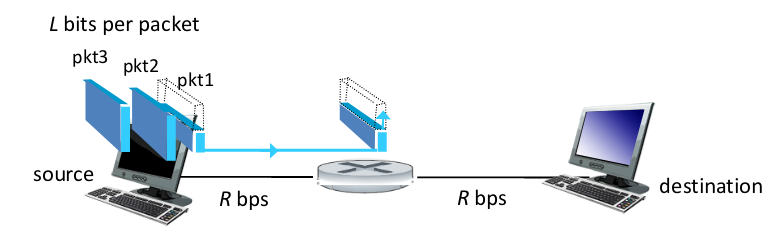
\includegraphics[scale=0.7]{packet-switching}
\begin{itemize}
	\item Takes L/R seconds to transmit (push out) L-bit packet into link at R bps
	\item Store and forward: \textbf{entire packet} must arrive at router before it can be transmitted on next link
	\item End-end delay = 2L/R (assuming zero propagation delay)
\end{itemize}
\subsection{Queuing delay, loss}
\begin{center}
	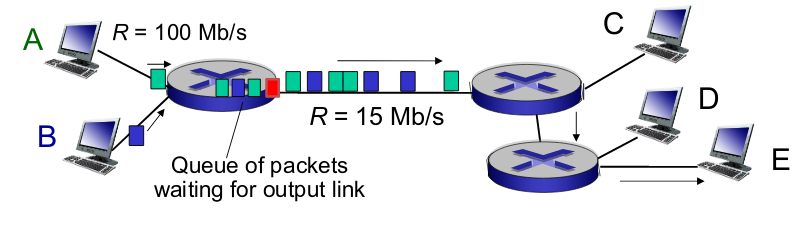
\includegraphics[scale=0.7]{queue}
\end{center}
If arrival rate (in bits) to link exceeds transmission rate of link for a period of time
\begin{itemize}
	\item Packets will queue, wait to be transmitted on link
	\item Packets can be dropped (lost) if memory (buffer) fills up
\end{itemize}
\section{Two key network-core functions}
\textbf{Routing}: Determines source-destination route taken by packets\\
\textbf{Forwarding}: Move packets from router's input to appropriate router output
\section{How do loss and delay occur?}
Packets queue in router buffers
\begin{itemize}
	\item Packet arrival rate to link (temporarily) exceeds output link capacity
	\item Packets queue, wait for turn
\end{itemize}
\begin{center}
	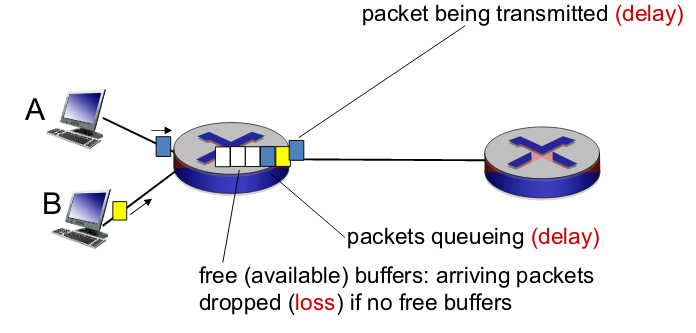
\includegraphics[scale=0.7]{loss}
\end{center}
\section{Four sources of packet delay}
\begin{center}
	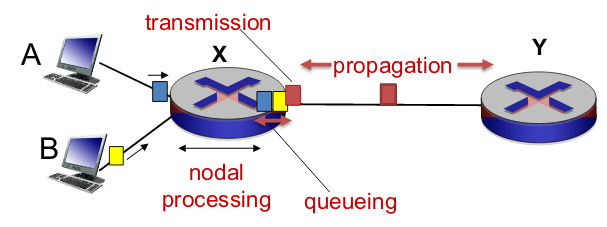
\includegraphics[scale=0.7]{loss1}
\end{center}
{\Large
$$d_{nodal}=d_{proc}+d_{queue}+d_{trans}+d_{prop}$$}
$d_{proc}$: nodal processing (delay in one router to process the packet)
\begin{itemize}
	\item Check bit errors
	\item Find information to determine where to send packet
	\item Determine output link
	\item Typically $<$ msec
\end{itemize}
$d_{queue}$: queuing delay
\begin{itemize}
	\item Time waiting at output link for transmission
	\item Depends on congestion level of router
\end{itemize}
$d_{trans}$: Transmission delay
\begin{itemize}
	\item How long it takes the packet to get out of the router
	\item L: Packet length (bits)
	\item R: Link bandwidth (bps)
	\item $d_{trans}$=L/R
\end{itemize}
$d_{prop}$: Propagation delay:
\begin{itemize}
	\item Time for transmission of data between the routers
	\item d: length of physical link
	\item s: propagation speed ($\sim 2\times 10^8 m/s$)
	\item $d_{prop}=d/s$
\end{itemize}
\subsection{Caravan Analogy}
\begin{center}
	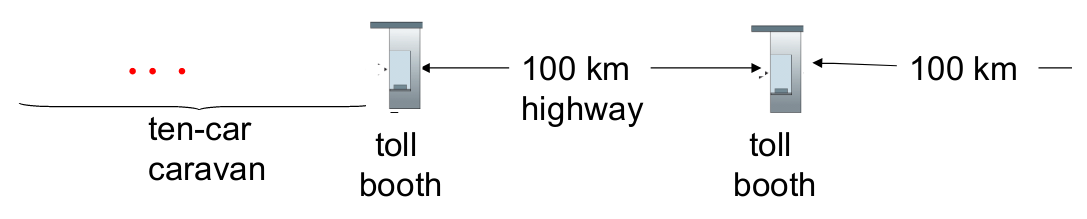
\includegraphics[scale=0.6]{caravan}
\end{center}

Cars "propagate" at
\begin{itemize}
	\item 100 km/hr
	\item Toll booth takes 12 seconds to service car (bit transmission)
	\item car $\sim$ bit; caravan $\sim$ packet
\end{itemize}
\textit{These caravans aren't actually caravans, instead a group of cars}\\
\\
Time to "push" entire caravan through toll booth onto highway=$12\times 10=120$ seconds\\
\\
Time for last car to propagate from 1st to 2nd toll booth =1hr
\section{Packet Loss}
\begin{itemize}
	\item Queue (aka buffer) preceding link in buffer has finite capacity
	\item Packet arriving to a full queue dropped (aka lost)
	\item Lost packet may be retransmitted by previous node, bu source end system, or not at all
\end{itemize}
\begin{center}
	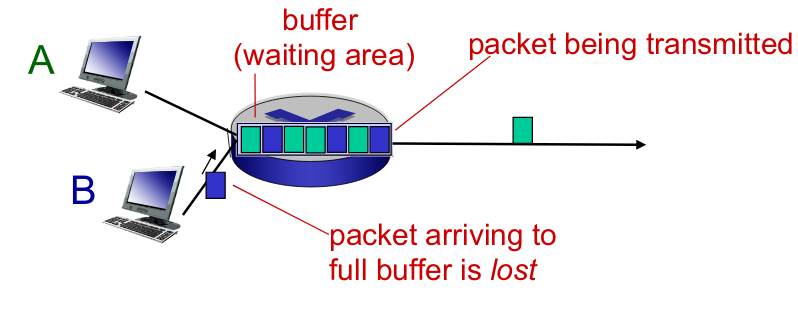
\includegraphics[scale=0.7]{packet_loss}
\end{center}
\section{"Real" internet delays and routes}
\begin{itemize}
	\item What do "real" internet delay \& loss look like?
	\item \texttt{traceroute} program: provides delay measurement from source to router along end-end internet path towards destination. For all i:
	\begin{itemize}
		\item Sends three packets to router i on path towards destination
		\item Router i will return packets to sender
		\item Sender times interval between transmission and reply
	\end{itemize}
\end{itemize}
\begin{center}
	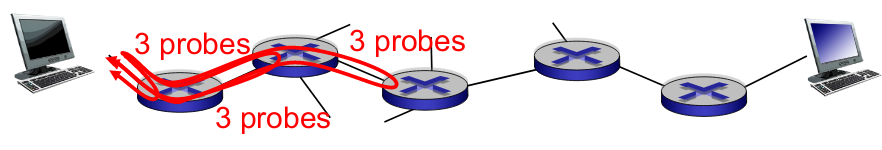
\includegraphics[scale=0.7]{delay_and_routes}
\end{center}
\section{Alternative core: circuit switching}
\begin{center}
	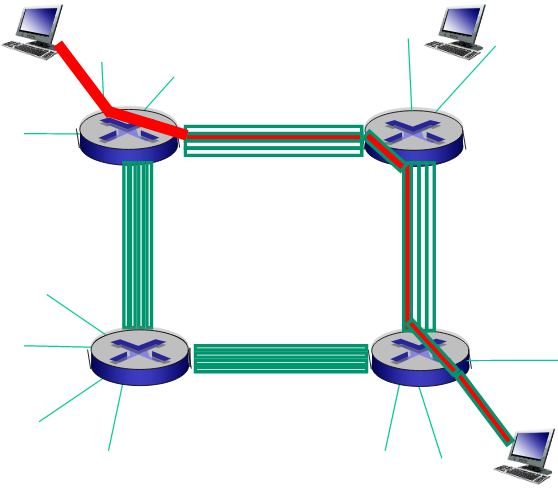
\includegraphics[scale=0.7]{circuit_switching}
\end{center}
End resources allocated to, reserved for "call" between source and destination
\begin{itemize}
	\item In diagram, each link has four circuits. Call gets 2nd circuit in top link and 1st circuit in right link
	\item Dedicated resources: no sharing. Circuit-like (guaranteed) performance
	\item Circuit segment idle if not being used by call (no sharing)
	\item Commonly used in traditional telephone networks
\end{itemize}
\section{Protocol "layers"}
Protocols determine the format and order of messages between devices. Protocol layering has conceptual and structural advantages.\\
\textbf{Protocol Stack}: Protocols of the various layers
\subsection{Why layering?}
Dealing with complex systems:
\begin{itemize}
	\item Explicit structure allows identification, relationship of complex system's pieces
	\item Modularization eases maintenance, updating of system
	\begin{itemize}
		\item Change of implementation of layer's service transparent to rest of system
	\end{itemize}
\end{itemize}
\subsection{Internet Protocol Stack}
\begin{minipage}{0.7\textwidth}
\begin{itemize}
	\item \textbf{Application}: Supporting network applications
	\begin{itemize}
		\item FTP, SMTP, HTTP
	\end{itemize}
	\item \textbf{Transport}: process-process data transfer
	\begin{itemize}
		\item TCP, UDP
	\end{itemize}
	\item \textbf{Network}: Routing of datagrams from source to destination
	\begin{itemize}
		\item IP, Routing Protocols
	\end{itemize}
	\item \textbf{Link}: Data transfer between neighbouring network elements
	\begin{itemize}
		\item Ethernet, 802.11, PPP
	\end{itemize}
	\item \textbf{Physical}: Bits "on the wire"
\end{itemize}
\end{minipage}
\begin{minipage}{0.3\textwidth}
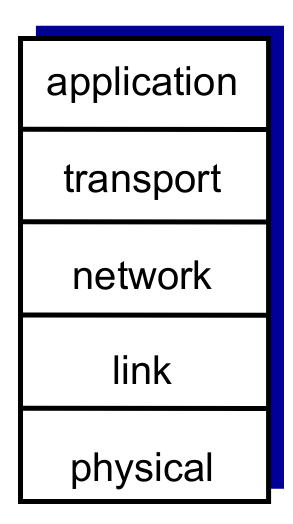
\includegraphics[scale=0.5]{IP_Stack}
\end{minipage}
\subsection{ISO/OSI Reference Model}

\begin{minipage}{0.7\textwidth}
\begin{itemize}
	\item \textbf{Presentation}: allow applications to interpret meaning of data e.g. encryption, compression, machine specific conventions
	\item \textbf{Session}: Synchronization, checkpointing, recovery of data exchange
	\item Internet stack "missing" these layers. These services if needed must be implemented in application
\end{itemize}
\end{minipage}
\begin{minipage}{0.3\textwidth}
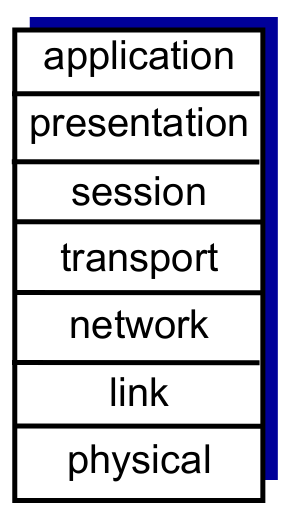
\includegraphics[scale=0.5]{OSI}

\end{minipage}

\end{document}